% Nicholas R. Jenkins
% Article
% Nicholas R. Jenkins (nicholas.jenkins@email.ucr.edu)
% Department of Political Science
% University of California, Riverside
%
% Manuscript: Minimizing Whose Influence? How Rejecting PAC Contributions Affects Contribution Patterns


% Setup Document and Formatting %
\documentclass[12pt]{article}


\usepackage[utf8]{inputenc}
\usepackage{hyperref}
\usepackage{setspace}
\usepackage[margin=1in]{geometry}
\usepackage[dvipsnames]{xcolor}
\usepackage{bookmark}
\usepackage[english]{babel}
\usepackage{csquotes}
\usepackage{fancyhdr}
\usepackage[bottom]{footmisc}
\usepackage[titletoc,title]{appendix}
\usepackage{tikz}
\usetikzlibrary{positioning}
\usepackage{tabu}
\usepackage{graphicx}
\usepackage{booktabs}
\usepackage{amsfonts}
\usepackage{pdflscape}
\usepackage{footmisc}
\usepackage{caption}
\usepackage{subcaption}
\usepackage{ntheorem}
\usepackage{amsmath}
\usepackage{bm}
\usepackage{longtable}
\usetikzlibrary{shapes, shadows, arrows}
\usepackage{rotating}
\usepackage{multirow}
\usepackage[section]{placeins}
\usepackage{pgfplots}



% Reference Setup %
\hypersetup{
    pdftitle={},    			% title
    pdfauthor={Nicholas R. Jenkins},     		% author
    pdfsubject={},   		% subject of the document
    pdfkeywords={}, 	% list of keywords
    pdfnewwindow=true,      		% links in new window
    colorlinks=false,       			% false: boxed links; true: colored links
    linkcolor=blue,          			% color of internal links
    citecolor=blue,        			% color of links to bibliography
    filecolor=blue,      				% color of file links
    urlcolor=blue           			% color of external links
}


% Bibliography Setup %
\usepackage[authordate, natbib, isbn=false, url=false, doi=false, backend=biber]{biblatex-chicago} 
\bibliography{/Users/nick/Documents/Research/References/BibTeX/biblatex.bib}
    
\DeclareCiteCommand{\citeauthorfirstlast}
  {\boolfalse{citetracker}%
   \boolfalse{pagetracker}%
   \DeclareNameAlias{labelname}{first-last}%
   \usebibmacro{prenote}}
  {\ifciteindex
     {\indexnames{labelname}}
     {}%
   \printnames{labelname}}
  {\multicitedelim}
  {\usebibmacro{postnote}}


% Hypotheses %
\newtheorem{hyp}{Hypothesis}

\makeatletter
\newcounter{subhyp} 
\let\savedc@hyp\c@hyp
\newenvironment{subhyp}
 {%
  \setcounter{subhyp}{0}%
  \stepcounter{hyp}%
  \edef\saved@hyp{\thehyp}% Save the current value of hyp
  \let\c@hyp\c@subhyp     % Now hyp is subhyp
  \renewcommand{\thehyp}{\saved@hyp\alph{hyp}}%
 }
 {}
\newcommand{\normhyp}{%
  \let\c@hyp\savedc@hyp % revert to the old one
  \renewcommand\thehyp{\arabic{hyp}}%
} 
\makeatother


% Title Page Setup %
\title{\textbf{Minimizing Whose Influence? How Rejecting PAC Contributions Affects Contribution Patterns}}

% Solo Author
\author{Nicholas R. Jenkins \\ Department of Political Science\\ University of California, Riverside\\ \href{mailto:nicholas.jenkins@email.ucr.edu}{nicholas.jenkins@email.ucr.edu}}

\date{\today}


% Document %
\begin{document}

% Title Page %
\maketitle
\thispagestyle{empty}

\begin{abstract}
% concisely describe the problem and your solution to it (or the question and your answer to it) and explain why this is a novel contribution. Carefully draft each sentence in the abstract to efficiently convey all the important information about your paper

Do pledges to reject corporate PAC contributions minimize corporate influence in elections? I address this question with campaign finance data for Congressional candidates in the 2018 elections. Using a zero-augmented gamma likelihood function to model the data generation process, I find that candidates who pledge to reject corporate PAC contributions are expected to receive fewer contributions from ideological, labor, and business PACs. Additionally, they are expected to receive more small-dollar contributions, large-dollar contributions, and contributions from individuals affiliated with business interests. These findings suggest that voters are motivated to donate by anti-PAC pledges as candidates hope, but that rather than minimizing their contribution activities, corporations use alternative contribution strategies for these candidates. This study is the first to examine the effects of rejecting PAC contributions on contribution patterns, and the first test of the claim that anti-PAC pledges will increase small-dollar donations.

\medskip

\noindent \textbf{Key Words:} Campaign Finance; Elections; Political Action Committees; Small Donors

\end{abstract}

\pagebreak

\cleardoublepage
\setcounter{page}{1}

\doublespacing

% Section 1: Introduction  %
\section{Introduction} \label{sec: intro}

On national television during the Democratic debate on February 6, 2016, Bernie Sanders stood on stage and enthusiastically announced to the audience, ``I am very proud to be the only candidate up here who does not have a super PAC, who’s not raising huge sums of money from Wall Street and special interests." Indeed, during the campaign, Sanders publicly voiced his opposition to Political Action Committee (PAC) contributions and refused to accept their donations while his Democratic opponent, Hillary Clinton, accepted over \$1.7 million from PACs; a decision for which she faced sharp criticism from voters on the left \citep{seitz-wald2015, bump2016}. 

This trend in rejecting PAC contributions has continued into the 2018 Congressional races and the 2020 presidential races. \citet{evers-hillstrom2018} reported in OpenSecrets News that 52 members of the 116 Congress, including 35 non-incumbents, announced that they would not accept money from corporate PACs during their campaigns. Similarly, \citeauthorfirstlast{harper2019} \citeyearpar{harper2019} wrote an article in ABC News claiming, ``The 2020 Democratic presidential candidates are forgoing corporate money in an effort to capture small donors.'' As of April of 2019, all 14 of the 2020 presidential Democratic candidates have declined to accept corporate PAC contributions (although only three have declined to accept contributions from all PACs). 

The push for campaign donations in the form of small-dollar donations, rather than PAC contributions, is indicative of demand from, or at least a perception among candidates of, voters wanting to bring the era of ``captured" politicians to an end \citep{culberson2019}. Indeed, the implicit belief seems to be that contributions from PACs affiliated with corporations produce corruption and render elected officials unwilling to serve the public interest. ``We desperately need to get the money out of the political system. Because I don’t think we have a Congress that’s representing the people anymore," a Minnesota resident complained during the 2018 midterm \citep{stockman2018}. When asked about his decision to reject PAC money, Beto O’Rourke's communications director said, ``It’s a major theme of the campaign. People want to know that you are going to respond to them and their interests, and not the most recent check you received" \citep{stockman2018}. 

Despite the stated intentions of anti-PAC pledges, do they limit corporations' influence in elections? I argue that while anti-PAC pledges signal a candidate's trustworthiness to voters, thus motivating them to make small-dollar contributions, corporations pursue alternative contribution strategies for candidates who make this pledge rather than cease their contribution activity altogether. Using Federal Election Commission data on campaign donations for Democratic candidates in the 2018 Congressional House Election, I show that candidates who reject PAC contributions are expected to receive more individual contributions of less than \$200, which supports the claim that voters approve of anti-PAC pledges and are responsive to candidates' efforts to get-out-the-small-dollar-donations. 

Additionally, I show that while candidates who make anti-PAC pledges are predicted to receive fewer PAC contributions, they are also expected to receive more money from large-dollar individual contributions and contributions from individuals affiliated with ideological and business interests. These increases suggest that although anti-PAC pledges may reduce PAC influence, they still allow corporate influence via individual donations. 

This study makes two significant contributions. First, to my knowledge, it is the first to examine the effects of pledging to reject PAC contributions on the distribution of a candidate's campaign contributions. Campaign finance is an omnipresent concern for the vast majority of voters and political scientists, thus refusing PAC donations presents a curious strategy with unknown consequences. In order to continue making progress in our understanding of how money is used to influence politics, we must investigate the evolving strategies of making and soliciting contributions.  

Second, this study is the first to test the claim that candidates will increase the amount of small-dollar donations from individual voters by pledging to reject corporate PAC contributions. The trend of candidates refusing to accept campaign contributions from PACs suggests that candidates assume this fact and that they also believe that they will attract more small-dollar donations from individuals by publicizing their opposition to PACs.  


\section{Voter Perceptions and Corporate Influence}

Whether a candidate would reject corporate PAC contributions as a matter of principle or electoral strategy is challenging to know. It is, however, undoubtedly the case that Americans are skeptical about money in politics \citep{lubenow2001}. Voters typically perceive contributions made by corporations as more corrupt than those made by individuals and consider small-dollar contributions as the most honest \citep{bowler2016}. Thus, the sources of campaign funding matter to voters, and attempts to distance oneself from ``corrupt" sources may prove electorally advantageous. 

In effect, making an anti-PAC pledge may serve as a signal of a more ``trustworthy" candidate. Indeed, these types of signaling effects have been well-documented \citep{iyengar1989}. Ella \citet{nilsen2019} reported that Elizabeth Warren ``swore off PAC money to make a statement" in a story for Vox.com. In an email to her supporters, Warren explained, ``For every time you see a presidential candidate talking with voters at a town hall, rally, or local diner, those same candidates are spending three or four or five times as long with wealthy donors — on the phone, or in conference rooms at hedge fund offices, or at fancy receptions and intimate dinners — all behind closed doors" \citep{nilsen2019}. The 2020 Democratic candidates are almost in a competition to distance themselves as far as they can from PACs and special interests, and there is little reason to suspect that the 2018 Democratic Congressional candidates would view this issue any differently. 

Rejecting corporate PAC contributions may motivate individual small donors, but whether it also meets the stated goal of reducing corporate influence is unclear. Campaign costs are enormous and continually rising, meaning that candidates who forgo contributions from corporate PACs will need to recover these lost funds from other sources. Moreover, given the opportunity costs corporations face from not getting involved in an election \citep{denzau1986, grier1986, kroszner1998}, it would be economically irrational for a corporate PAC interested in influencing politics to abandon its efforts because a candidate wishes to avoid the negative publicity of receiving contributions from corporate PACs. Instead, a rational corporate PAC should use alternative means to make campaign contributions. 

One such alternative is to fund candidates directly with large-dollar donations and corporately-bundled individual donations. Indeed, the Center for Responsive Politics documents donations made by individuals in connection with larger organizations because, ``In some cases, a cluster of contributions from the same organization may indicate a concerted effort by that organization to `bundle' contributions to the candidate." Such a strategy would allow recipients to claim that they do not accept corporate PAC money while still receiving corporate support. 


\section{Data, Methods, and Results}

To evaluate anti-PAC pledges, I take advantage of unique campaign finance data on Congressional candidates in the 2018 midterm election provided by The Center for Responsive Politics at \href{https://www.opensecrets.org}{Opensecrets.org.} The data are unique because The Center for Responsive Politics is the first organization, to my knowledge, to keep records on which candidates pledged not to accept corporate PAC contributions for the 2018 elections. Unfortunately, this limits my sample to only the 2018 midterm. This cross-section makes it challenging to generalize model results beyond one election, but I believe that these data still provide a foundation for meaningful results, especially since the pattern of refusing corporate PAC contributions has continued in subsequent elections.    

In the available data on candidates who refuse corporate PAC contributions, data are only provided for candidates who won their elections. While this does limit the sample, it also helps to create better comparison groups. It is necessarily the case that candidates that did not win their elections differ, likely systematically, from those that did win, and these differences could be on factors that also determine campaign contributions. By excluding candidates who lost their election in the sample, these differences are effectively controlled. I do restrict, however, the sample only to include Democrats. Since the composition of campaign contributors differs between parties, only including Democrats helps remove some of this heterogeneity. Moreover, refusing corporate PAC money is not a common strategy among Republicans; only 2 Republicans in the sample took the pledge to reject corporate PAC contributions. The final sample contains 167 Democratic candidates that won election in their district. 

\begin{figure}[!htb]
    \centering
    \includegraphics[width=0.90\linewidth]{../../Figures/all_candy.pdf}
    \caption{Contributions to Candidates by Source and Whether or not they Reject PAC Contributions.}
    \label{fig: all contribs}
\end{figure}

Figure \ref{fig: all contribs} displays the mean contributions across candidates by whether or not they pledge to reject corporate PAC contributions. We see that candidates who pledge to reject corporate PAC contributions receive almost zero contributions from business PACs, and they also receive much fewer contributions from PACs in total. However, these candidates also receive more contributions from individuals affiliated with ideological interest groups, small-dollar donations, individuals affiliated with business interest groups, and large-dollar donations. Interestingly, candidates who reject corporate PAC contributions far outspend and outraise their corporate PAC accepting counterparts, as shown in Figure \ref{fig: spending}.

\begin{figure}[ht]
    \centering
    \includegraphics[width=0.90\linewidth]{../../Figures/spending_candy.pdf}
    \caption{Mean Candidate Spending and Receipts by Whether or not they Reject PAC Contributions.}
    \label{fig: spending}
\end{figure}

To describe the data generating process of campaign contributions, I use a gamma likelihood function since the gamma distribution describes a data generating process for a random variable with only positive real number outcomes $y \in  \mathbb{R}^+$. However, because some candidates pledge to reject PAC contributions, contribution values of zero are also possible.\footnote{See Figure \ref{fig: zeros} in the Appendix for a visualization of the percentage of zeros in the data.} A zero could result because they accept zero contributions from a group, but a group could also decide not to contribute to a candidate because they pledged to reject PAC contributions. 

\begin{figure}[!htb]
    \centering
    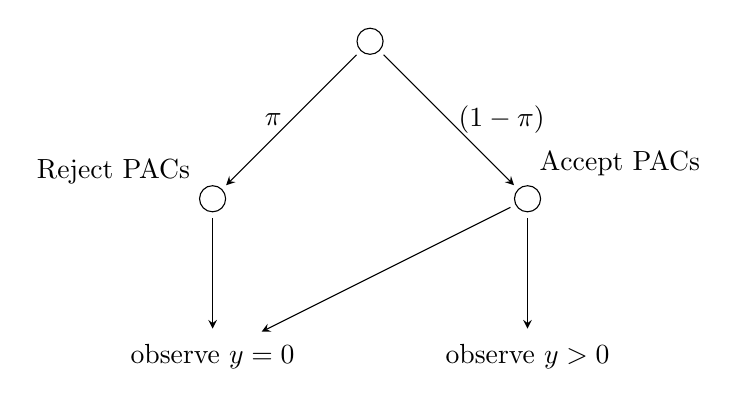
\begin{tikzpicture}[
        node distance=2.0cm,
      scale=0.5,
      level/.style={thick},
      virtual/.style={thick,densely dashed},
      trans/.style={->,shorten >=2pt,shorten <=2pt,>=stealth},
      classical/.style={thin,double,<->,shorten >=4pt,shorten <=4pt,>=stealth}
    ]
    \node(a)[circle, draw=black, label={160:Reject PACs}] {};
    \node(z)[right of=a] {};
    \node(b)[circle, draw=black, right of=z, label={80:Accept PACs}] {};
    \node(c)[circle, draw=black, above of=z] {};
    \node(d)[below of=a] {observe $y = 0$};
    \node(e)[below of=b] {observe $y > 0$};
    
    \draw [trans] (c) -- (a) node[midway, left] {$\pi$};
    \draw [trans] (c) -- (b) node[midway, right] {$(1 - \pi)$};
    \draw [trans] (a) -- (d);
    \draw [trans] (b) -- (e);
    \draw [trans] (b) -- (d);
    \end{tikzpicture}
    \caption{Zero Generation Process.}
    \label{fig: zero process}
\end{figure}

This dual process is summarized in Figure \ref{fig: zero process}. Candidates decided to reject PACs with a probability of $\pi$ or accept PACs with probability $(1 - \pi$). If they reject PACs, we will observe a zero. If they accept PAC contributions, we may still observe a zero if the candidate fails to attract donations from the group in question. Because the gamma distribution is not defined for zero values, I use a zero-augmented gamma likelihood function for models of contributions that contain zero values as mentioned above. The zero-augmented gamma likelihood is a mixture of a bernoulli and gamma process. Thus, the probability density $f(y)$ for contributions can be defined as:    

\begin{align}
f(y) = \left\{ \begin{array}{cc} 
                \pi & \hspace{5mm} \text{if $y = 0$} \\
                (1 - \pi) \text{Gamma}(k, \theta) & \hspace{5mm}  \text{if $y > 0$} \\
                \end{array} \right.
\end{align}

\noindent where $\pi$ is the probability of receiving zero contributions from a given group ($y = 0$), and $k$ and $\theta$ define a gamma distribution with mean $k\theta^{-1}$ and rate $\theta$. This likelihood can be easily summarized as $\text{ZGamma}(\pi, \mu, \theta)$ where $\pi$ indicates the probability of a zero, and non-zero outcomes are described by a mean $\mu$ and rate $\theta$.\footnote{For more information on the mathematical details, see \citet{mccullagn1989}} An alternative solution to model this data would be to model cases of zero contributions separately from non-zero cases, but this approach would sacrifice information about the relationship between these cases. By leaving zero cases in the dataset, the model can allow the probability of observing a zero inform the coefficient estimates in the gamma likelihood and vice versa. This way, the model can develop a more accurate picture of the data generating process. The model structure used to estimate campaign contributions for outcomes that contain zeros is given by: 

$$
\begin{aligned}
    y_i &\sim \text{ZGamma}(\pi_i, \mu_i, \theta_i) \\
    \log \left( \frac{\pi_i}{1 - \pi_i} \right) &= \alpha_{\pi} + \beta_{1\pi} (\text{No PACs})_i + \beta_{2\pi} (\text{New Member})_i \\
    \log(\mu_i) &= \alpha_{\mu} + \beta_{1\mu} (\text{No PACs})_i + \bm{X} \bm{\beta_{\mu}} \\
\end{aligned}
$$

\noindent where $i$ indexes individuals, $\bm{X}$ is a matrix of adjustment variables, and $\bm{\beta_{\mu}}$ is the corresponding coefficient vector. In these models, the probability of receiving contributions is modeled as a function of both rejecting PACs (0 - 1 indicator) and being a new member (0 - 1 indicator). Previous research indicates that PACs almost exclusively contribute to incumbents \citep{brunell2005} and often wait to support challengers until they show success in raising funds from other sources \citep{biersack1993}. 

To model campaign contributions for outcomes without zeros (small-dollar individual, large-dollar individual, business individual, total individual), I use a standard gamma likelihood. All models are estimated with weakly-informative priors to better approximate large-n estimates \citep{mcneish2016} and because using ``uninformative" priors is seldom justified since one always knows something \textit{a priori} about the range of plausible values \citep{gelman2008a}. For simulations of the priors used in each specification, see Appendix \ref{sec: prior sims}.

\begin{figure*}[!htb]
        \centering
        \includegraphics[width=0.75\linewidth]{pac_coef.pdf}
        \caption{The Effect of Rejecting Corporate PAC Contributions on PAC Contributions.}
        \label{fig: pac coefs}
\end{figure*}

Figure \ref{fig: pac coefs} shows that when comparing candidates with the same values for all the adjustment variables but who differed on whether they accept corporate PAC contributions, the models predict candidates who reject corporate PAC contributions to have fewer PAC contributions from business, labor, and ideological PACs.\footnote{See Table \ref{tbl: pac results} in the Appendix \ref{sec: reg tables} for the complete table of results.} Although it is not entirely clear why contributions from labor and ideological PACs would decrease contributions, the reduction in business PAC contributions is expected.

Next, I investigate if anti-PAC pledges are associated with increases in small-dollar donations. Remarkably, Figure \ref{fig: indiv coefs} shows that candidates who reject corporate PACs are predicted to receive an expected 90 percent increase in contributions from donors who gave less than \$200.\footnote{See Table \ref{tbl: indiv results} in Appendix \ref{sec: reg tables} for the complete table of results.} This finding supports the claim that voters are motivated to donate to candidates who take a stand to reduce corporate money in the political system. 

Finally, I investigate whether corporations bundle individual donations to continue supporting candidates that make anti-PAC pledges. Supporting this claim, Figure \ref{fig: indiv coefs} shows that campaign contributions from individuals affiliated with businesses, ideological organizations, and large-dollar contributions are expected to be higher for candidates who reject corporate PAC contributions than for candidates who accept contributions from corporate PACs.\footnote{These results are also shown in Table \ref{tbl: indiv results} of Appendix \ref{sec: reg tables}.}

\begin{figure*}[!htb]\centering
        \includegraphics[width=0.75\linewidth]{indv_coef.pdf}
        \caption{The Effect of Rejecting Corporate PAC Contributions on Contributions from Individuals.}
        \label{fig: indiv coefs}
\end{figure*}

These results suggest that anti-PAC pledges are associated with increased support from small-dollar donations, which bolsters the claim that voters are motivated to get money out of politics and support candidates they believe are making efforts to accomplish this objective. However, these results also indicate that anti-PAC pledges may not reduce corporate influence in elections as much as some might have hoped. Instead, these pledges are associated with alternative corporate contribution strategies. Rather than abandon their efforts to influence politics, corporations continue to support candidates who refuse corporate PAC money by making bundled donations through individuals.


\section{Conclusion} \label{sec: conclusion}

The recent trend of Congressional and presidential candidates rejecting corporate PAC contributions is a puzzling campaign strategy that has yet to receive much academic investigation. Although candidates advertise this strategy as an attempt to finance their campaigns with small-dollar individual donations, it is unclear whether it is successful in accomplishing this goal or whether it reduces corporate influence. 

In this paper, I offer evidence that anti-PAC pledges do galvanize small-dollar donations but that they may not reduce corporate influence. Instead, anti-PAC pledges are associated with alternative corporate contribution strategies. Specifically, I find that candidates who reject corporate PAC contributions are predicted to receive fewer contributions from business PACs, but they are also predicted to receive more contributions from individuals affiliated with businesses and large-dollar individual donations.  

This study is limited to just one Congressional election, 2018, so future work will is needed to determine whether these findings can be generalized to other elections. However, so far into the 2020 elections, an increasing number of Democratic candidates are rejecting corporate PAC contributions and doubling down on their solicitation of small-dollar donations. If we are to develop a stronger understanding of how money is used to influence the political process, we must continue investigating the evolving ways in which individuals and groups make contributions as well as how members solicit contributions. 

\singlespacing
\pdfbookmark[1]{References}{References}
%\bibliography{/Users/nick/Documents/Research/Articles/reference.bib}
\printbibliography
\pagebreak


\begin{appendices}
\doublespacing
% Set Tables Names to have "A" Before the Table Names
\setcounter{table}{0}
\renewcommand{\thetable}{A\arabic{table}}

\section{Data}

Figure \ref{fig: zeros} shows the percentage of zeros in the data. Of the 167 candidates in the data, 84 percent did not receive contributions from party committees, 68 percent did not receive contributions from individuals affiliated with labor organizations, 12 percent did not receive contributions from candidate committees, 10 percent did not receive contributions from leadership PACs, 5 percent did not receive contributions from business PACs,  4 percent did not receive contributions from individuals affiliated with ideological organizations, 2 percent did not receive contributions from labor PACs, and 1 percent did not receive contributions from ideological PACs and PACs in general.  

\begin{figure}[!htb]
    \centering
    \includegraphics[width=0.85\linewidth]{zero_candy.pdf}
    \caption{Percentage of Zero Contributions in the Data by Source of Contribution.}
    \label{fig: zeros}
\end{figure}


\section{Results Tables} \label{sec: reg tables}


\begin{table}[h]
\begin{center}
\caption{The Effects of Pledging to Reject Corporate PAC contributions on Contributions from PACs}
\label{tbl: pac results}
\resizebox{\columnwidth}{!}{%
\setlength{\linewidth}{.1cm}\newcommand{\contents}{\begin{tabular}{@{\extracolsep{5pt}}l c c c c }
 \\[-1.8ex] \toprule  \\[-1.8ex]
 & \multicolumn{4}{c}{\textbf{Outcome Variable:}} \\
\textbf{Predictor Variables} & Total PAC \$ & Business PAC \$ & Ideological PAC \$ & Labor PAC \$ \\
 \midrule  \\[-1.8ex]
\\[-1.8ex] \textit{Gamma Model (log link)} \\
\midrule  \\[-1.8ex]
 \\[-1.8ex] \textit{Predictor of Interest} \\  \\[-1.8ex]
	\quad No to Corporate PAC Contributions     & $-0.79^{*}$               & $-2.02^{*}$               & $-0.13^{*}$             & $-0.51^{*}$             \\
          & $[-0.84;\ -0.74]$         & $[-2.17;\ -1.88]$         & $[-0.18;\ -0.06]$       & $[-0.57;\ -0.45]$       \\
\\[-1.8ex] \textit{Controls} \\ \\[-1.8ex]
	\quad New Member    & $-1.04^{*}$               & $-2.41^{*}$               & $0.68^{*}$              & $-0.41^{*}$             \\
          & $[-1.07;\ -1.00]$         & $[-2.49;\ -2.32]$         & $[0.61;\ 0.74]$         & $[-0.46;\ -0.36]$       \\
	\quad \% of White Population in District  & $-0.00$                   & $-0.01^{*}$               & $-0.04^{*}$             & $0.01^{*}$              \\
          & $[-0.00;\ 0.00]$          & $[-0.01;\ -0.01]$         & $[-0.05;\ -0.03]$       & $[0.01;\ 0.02]$         \\
	\quad \% of Black Population in District  & $-0.00$                   & $-0.00^{*}$               & $-0.04^{*}$             & $0.00$                  \\
          & $[-0.01;\ 0.00]$          & $[-0.01;\ -0.00]$         & $[-0.05;\ -0.04]$       & $[-0.01;\ 0.01]$        \\
	\quad \% of Latino Population in District & $-0.00$                   & $-0.01^{*}$               & $-0.03^{*}$             & $0.00$                  \\
          & $[-0.01;\ 0.00]$          & $[-0.01;\ -0.01]$         & $[-0.03;\ -0.02]$       & $[-0.00;\ 0.01]$        \\
	\quad \% of Asian Population in District  & $-0.02^{*}$               & $-0.01^{*}$               & $-0.05^{*}$             & $-0.01^{*}$             \\
          & $[-0.02;\ -0.02]$         & $[-0.02;\ -0.01]$         & $[-0.06;\ -0.04]$       & $[-0.01;\ -0.00]$       \\
	\quad \% of District Pop. with Bachelors Degree   & $-0.01^{*}$               & $-0.01^{*}$               & $0.00$                  & $-0.01^{*}$             \\
          & $[-0.01;\ -0.01]$         & $[-0.01;\ -0.01]$         & $[-0.00;\ 0.01]$        & $[-0.02;\ -0.01]$       \\
	\quad \% of District Vote for Clinton in 2016  & $-0.02^{*}$               & $-0.03^{*}$               & $-0.02^{*}$             & $0.01^{*}$              \\
          & $[-0.02;\ -0.01]$         & $[-0.03;\ -0.03]$         & $[-0.03;\ -0.02]$       & $[0.01;\ 0.02]$         \\
	\quad \% of District Vote for Dem. House Candidates in 2016  & $0.01^{*}$                & $0.01^{*}$                & $-0.00$                 & $-0.00^{*}$             \\
          & $[0.00;\ 0.01]$           & $[0.01;\ 0.01]$           & $[-0.00;\ 0.00]$        & $[-0.00;\ -0.00]$       \\
	\quad $\log$(Voting Age Population in District)   & $0.15$                    & $-0.05$                   & $1.32^{*}$              & $0.07$                  \\
          & $[-0.03;\ 0.33]$          & $[-0.28;\ 0.18]$          & $[0.83;\ 1.79]$         & $[-0.18;\ 0.30]$        \\
		\quad $\log$(Median Household Income)    & $0.64^{*}$                & $0.59^{*}$                & $0.29^{*}$              & $0.02$                  \\
          & $[0.57;\ 0.72]$           & $[0.50;\ 0.69]$           & $[0.10;\ 0.49]$         & $[-0.08;\ 0.13]$        \\
	\quad Intercept         & $13.33^{*}$               & $12.93^{*}$               & $10.07^{*}$             & $11.67^{*}$             \\
          & $[13.32;\ 13.34]$         & $[12.92;\ 12.95]$         & $[10.04;\ 10.10]$       & $[11.66;\ 11.69]$       \\ 
Dispersion Parameter     & $2514.54^{*}$             & $2363.02^{*}$             & $974.90^{*}$            & $1018.48^{*}$           \\
          & $[2475.14;\ 2554.93]$     & $[2323.03;\ 2400.76]$     & $[951.17;\ 1000.97]$    & $[992.44;\ 1043.38]$    \\
\\[-1.8ex] \textit{Binomial Model (Logit Link)} \\
\midrule  \\[-1.8ex]
\\[-1.8ex] \textit{Predictor of Interest} \\ \\[-1.8ex]
	\quad No to Corporate PAC Contributions     & $0.24$                    & $1.41^{*}$                & $-0.13$                 & $-0.00$                 \\
          & $[-1.07;\ 1.54]$          & $[0.43;\ 2.29]$           & $[-1.35;\ 1.14]$        & $[-0.20;\ 0.20]$        \\
\\[-1.8ex] \textit{Controls} \\ \\[-1.8ex]
	\quad New Member    & $-0.81$                   & $0.76$                    & $0.24$                  & $-0.01$                 \\
          & $[-2.19;\ 0.43]$          & $[-0.17;\ 1.69]$          & $[-0.89;\ 1.40]$        & $[-0.18;\ 0.16]$        \\
	\quad Intercept         & $-3.56^{*}$               & $-3.34^{*}$               & $-3.54^{*}$             & $-3.70^{*}$             \\
          & $[-4.33;\ -2.87]$         & $[-4.00;\ -2.70]$         & $[-4.28;\ -2.85]$       & $[-3.77;\ -3.63]$       \\
          \\
 \midrule  \\[-1.8ex]
Number of Observations & 167 & 167 & 167 & 167 \\
\bottomrule  \\[-1.8ex]
\multicolumn{5}{p{\linewidth}}{Notes: Models are estimated using zero-augmented Gamma likelihoods. Analyses use four Markov chain Monte Carlo (MCMC) chains at 10,000 iterations each with a warmup period of 5,000 samples using the Hamiltonian Monte Carlo algorithm. All chains indicate convergence with every \^{R} value being less than 1.01. Model coefficients are estimated with weakly informative priors. 89\% highest density intervals shown in brackets below each coefficient. $^*$ indicates that 0 is outside 89\% highest posterior density interval.}\\
\end{tabular}}
\setbox0=\hbox{\contents}
	\setlength{\linewidth}{\wd0-2\tabcolsep-.25em}
	\contents
}
\end{center}
\end{table}


\begin{landscape}
\begin{table}[!htb]
\begin{center}
\caption{The Effects of Pledging to Reject Corporate PAC contributions on Contributions from Individuals}
\label{tbl: indiv results}
\resizebox{\columnwidth}{!}{%
\setlength{\linewidth}{.1cm}\newcommand{\contents}{\begin{tabular}{@{\extracolsep{10pt}}l c c c c c c }
 \\[-1.8ex] \toprule  \\[-1.8ex]
 & \multicolumn{6}{c}{\textbf{Outcome Variable:}} \\
\textbf{Predictor Variables} & Small-dollar \$ & Large-dollar \$ & Total Indiv. \$ & Ideological Indiv. \$ & Business Indiv. \$ & Labor Indiv. \$\\
 \midrule  \\[-1.8ex]
\\[-1.8ex] \textit{Gamma Model (log link)} \\
\midrule  \\[-1.8ex]
 \\[-1.8ex] \textit{Predictor of Interest} \\  \\[-1.8ex]
\quad No to Corporate PAC Contributions     & $0.65^{*}$                & $0.26^{*}$                & $0.34^{*}$                & $0.27^{*}$              & $0.08^{*}$                & $0.04$                \\
          & $[0.61;\ 0.69]$           & $[0.24;\ 0.28]$           & $[0.32;\ 0.36]$           & $[0.21;\ 0.32]$         & $[0.05;\ 0.12]$           & $[-0.20;\ 0.28]$      \\
\\[-1.8ex] \textit{Controls} \\ \\[-1.8ex]
	\quad New Member     & $0.99^{*}$                & $0.63^{*}$                & $0.69^{*}$                & $0.63^{*}$              & $0.14^{*}$                & $1.07^{*}$            \\
          & $[0.94;\ 1.04]$           & $[0.60;\ 0.66]$           & $[0.66;\ 0.71]$           & $[0.56;\ 0.70]$         & $[0.10;\ 0.18]$           & $[0.74;\ 1.39]$       \\
\quad \% of White Population in District  & $-0.04^{*}$               & $-0.01^{*}$               & $-0.01^{*}$               & $-0.06^{*}$             & $-0.00$                   & $-0.09^{*}$           \\
          & $[-0.04;\ -0.03]$         & $[-0.01;\ -0.00]$         & $[-0.01;\ -0.01]$         & $[-0.07;\ -0.05]$       & $[-0.01;\ 0.00]$          & $[-0.13;\ -0.06]$     \\
\quad \% of Black Population in District   & $-0.08^{*}$               & $-0.02^{*}$               & $-0.03^{*}$               & $-0.08^{*}$             & $-0.01^{*}$               & $-0.12^{*}$           \\
          & $[-0.09;\ -0.08]$         & $[-0.02;\ -0.02]$         & $[-0.03;\ -0.02]$         & $[-0.09;\ -0.07]$       & $[-0.02;\ -0.01]$         & $[-0.16;\ -0.09]$     \\
\quad \% of Latino Population in District & $-0.04^{*}$               & $0.00$                    & $-0.00$                   & $-0.04^{*}$             & $0.01^{*}$                & $-0.10^{*}$           \\
          & $[-0.04;\ -0.03]$         & $[-0.00;\ 0.01]$          & $[-0.00;\ 0.00]$          & $[-0.05;\ -0.04]$       & $[0.00;\ 0.01]$           & $[-0.13;\ -0.07]$     \\
\quad \% of Asian Population in District   & $-0.06^{*}$               & $-0.02^{*}$               & $-0.02^{*}$               & $-0.10^{*}$             & $-0.02^{*}$               & $-0.11^{*}$           \\
          & $[-0.06;\ -0.05]$         & $[-0.03;\ -0.02]$         & $[-0.03;\ -0.02]$         & $[-0.11;\ -0.09]$       & $[-0.02;\ -0.01]$         & $[-0.16;\ -0.06]$     \\
\quad \% of District Pop. with Bachelors Degree    & $-0.01^{*}$               & $-0.02^{*}$               & $-0.01^{*}$               & $-0.03^{*}$             & $-0.02^{*}$               & $0.05^{*}$            \\
          & $[-0.01;\ -0.01]$         & $[-0.02;\ -0.01]$         & $[-0.02;\ -0.01]$         & $[-0.03;\ -0.02]$       & $[-0.02;\ -0.01]$         & $[0.03;\ 0.07]$       \\
\quad \% of District Vote for Clinton in 2016  & $0.00^{*}$                & $-0.01^{*}$               & $-0.00^{*}$               & $0.01^{*}$              & $-0.01^{*}$               & $0.00$                \\
          & $[0.00;\ 0.01]$           & $[-0.01;\ -0.00]$         & $[-0.00;\ -0.00]$         & $[0.01;\ 0.01]$         & $[-0.01;\ -0.01]$         & $[-0.01;\ 0.02]$      \\
\quad \% of District Vote for Dem. House Candidates in 2016  & $-0.02^{*}$               & $-0.01^{*}$               & $-0.01^{*}$               & $-0.02^{*}$             & $-0.01^{*}$               & $0.04^{*}$            \\
          & $[-0.02;\ -0.01]$         & $[-0.01;\ -0.01]$         & $[-0.01;\ -0.01]$         & $[-0.02;\ -0.02]$       & $[-0.01;\ -0.01]$         & $[0.03;\ 0.05]$       \\
\quad $\log$(Voting Age Population in District)   & $-1.01^{*}$               & $0.28^{*}$                & $0.14$                    & $2.06^{*}$              & $1.15^{*}$                & $-2.69^{*}$           \\
          & $[-1.40;\ -0.62]$         & $[0.10;\ 0.45]$           & $[-0.02;\ 0.32]$          & $[1.63;\ 2.52]$         & $[0.92;\ 1.36]$           & $[-5.29;\ -0.15]$     \\
\quad $\log$(Median Household Income)    & $1.70^{*}$                & $2.14^{*}$                & $2.02^{*}$                & $3.67^{*}$              & $2.35^{*}$                & $-1.17^{*}$           \\
          & $[1.56;\ 1.83]$           & $[2.07;\ 2.21]$           & $[1.95;\ 2.09]$           & $[3.47;\ 3.86]$         & $[2.25;\ 2.44]$           & $[-1.97;\ -0.40]$     \\
\quad Intercept         & $10.87^{*}$               & $13.12^{*}$               & $13.26^{*}$               & $10.27^{*}$             & $12.48^{*}$               & $5.80^{*}$            \\
          & $[10.84;\ 10.91]$         & $[13.11;\ 13.13]$         & $[13.25;\ 13.28]$         & $[10.23;\ 10.31]$       & $[12.46;\ 12.49]$         & $[5.63;\ 5.99]$       \\
Dispersion Parameter     & $2269.58^{*}$             & $3737.15^{*}$             & $4093.77^{*}$             & $1589.96^{*}$           & $2658.35^{*}$             & $91.68^{*}$           \\
          & $[2230.23;\ 2305.61]$     & $[3689.42;\ 3787.57]$     & $[4042.55;\ 4143.86]$     & $[1559.06;\ 1621.54]$   & $[2617.04;\ 2699.94]$     & $[84.19;\ 98.85]$     \\
\\[-1.8ex] \textit{Binomial Model (Logit Link)} \\
\midrule  \\[-1.8ex]
\\[-1.8ex] \textit{Predictor of Interest} \\ \\[-1.8ex]
\quad No to Corporate PAC Contributions     &                           &                           &                           & $-0.82$                 &                           & $-0.38$               \\
          &                           &                           &                           & $[-2.15;\ 0.41]$        &                           & $[-1.07;\ 0.38]$      \\
\\[-1.8ex] \textit{Controls} \\ \\[-1.8ex]
	\quad New Member     &                           &                           &                           & $-0.50$                 &                           & $-0.17$               \\
          &                           &                           &                           & $[-1.64;\ 0.60]$        &                           & $[-0.79;\ 0.52]$      \\
 \quad Intercept        &                           &                           &                           & $-2.66^{*}$             &                           & $0.84^{*}$            \\
          &                           &                           &                           & $[-3.20;\ -2.14]$       &                           & $[0.53;\ 1.14]$       \\
 \midrule  \\[-1.8ex]
Number of Observations & 167 & 167 & 167 & 167 & 167 & 167 \\
\bottomrule  \\[-1.8ex]
\multicolumn{7}{p{\linewidth}}{Notes: Models are estimated using either a zero-augmented Gamma likelihood or a Gamma likelihood. Analyses use four Markov chain Monte Carlo (MCMC) chains at 10,000 iterations each with a warmup period of 5,000 samples using the Hamiltonian Monte Carlo algorithm. All chains indicate convergence with every \^{R} value being less than 1.01. Model coefficients are estimated with weakly informative priors. 89\% highest density intervals shown in brackets below each coefficient. $^*$ indicates that 0 is outside 89\% highest posterior density interval.}
\end{tabular}}
\setbox0=\hbox{\contents}
	\setlength{\linewidth}{\wd0-2\tabcolsep-.25em}
	\contents
}
\end{center}
\end{table}
\end{landscape}


\section{Prior Simulations} \label{sec: prior sims}

\begin{figure*}[!htb]
    \centering
    \begin{subfigure}[b]{0.45\textwidth}
        \centering
        \includegraphics[width=\linewidth]{pac_int.pdf}
        \caption{Priors for Model Intercepts}
    \end{subfigure}
    %
    \begin{subfigure}[b]{0.45\textwidth}
        \centering
        \includegraphics[width=\linewidth]{pac_slopes.pdf}
        \caption{Priors for Model Slopes}
    \end{subfigure}
    %
    \begin{subfigure}[b]{0.45\textwidth}
    	\centering
        \includegraphics[width=\linewidth]{pac_logit.pdf}
        \caption{Binomial Intercept \& Slope Priors}
    \end{subfigure}
    %
    \begin{subfigure}[b]{0.45\textwidth}
    	\centering
        \includegraphics[width=\linewidth]{pac_scale.pdf}
        \caption{Scale Parameter Priors}
    \end{subfigure}
    \caption{Priors for Parameters in PAC Contribution Models.}
    \label{fig: priors}
\end{figure*}

\begin{figure*}[!htb]
    \centering
    \begin{subfigure}[b]{0.45\textwidth}
        \centering
        \includegraphics[width=\linewidth]{indiv_int.pdf}
        \caption{Priors for Model Intercepts}
    \end{subfigure}
    %
    \begin{subfigure}[b]{0.45\textwidth}
        \centering
        \includegraphics[width=\linewidth]{indiv_slopes.pdf}
        \caption{Priors for Model Slopes}
    \end{subfigure}
    %
    \begin{subfigure}[b]{0.45\textwidth}
    	\centering
        \includegraphics[width=\linewidth]{pac_logit.pdf}
        \caption{Binomial Intercept \& Slope Priors}
    \end{subfigure}
    %
    \begin{subfigure}[b]{0.45\textwidth}
    	\centering
        \includegraphics[width=\linewidth]{pac_scale.pdf}
        \caption{Scale Parameter Priors}
    \end{subfigure}
    \caption{Priors for Parameters in Individual Contribution Models.}
    \label{fig: priors}
\end{figure*}


\end{appendices}


\end{document}
